% % % % % % % % % % % % % % % % % % % % % % % % % % % % % % % % % % % % % % % % % % % %
%                                                                                     %
% Short Sectioned Assignment LaTeX Template Version 1.0 (5/5/12)                      %
% This template has been downloaded from: http://www.LaTeXTemplates.com               %
%                                                                                     %
% Original author:  Frits Wenneker (http://www.howtotex.com)                          %
%                                                                                     %
% Modified by: Fco Javier Sueza Rodríguez (fcosueza@disroot.org)                      %
%                                                                                     %
% Changes:                                                                            %
%	    - Custom Chapters, Sections and Subsections (titlesec package)                %
%           - Document type scrbook (oneside)                                         %
%           - Use babel-lang-spanish package and marvosym                             %
%           - Use hyperref, enumitem, tcolorbox and glossaries packages               %
%           - Use Time New Roman (mathptmx), Helvetic and Courier fonts               %
%                                                                                     %
% License: CC BY-NC-SA 3.0 (http://creativecommons.org/licenses/by-nc-sa/3.0/)        %
%                                                                                     %
% % % % % % % % % % % % % % % % % % % % % % % % % % % % % % % % % % % % % % % % % % % %

%-----------------------------------------------%
%	              Packages                  %
%-----------------------------------------------%

\documentclass[paper=a4, fontsize=11pt, oneside]{scrbook}

% ---- Text Input/Output ----- %

\usepackage[T1]{fontenc}
\usepackage[utf8]{inputenc}
\usepackage{mathptmx}
\usepackage[scaled=.92]{helvet}
\usepackage{courier}
\usepackage[indent=12pt]{parskip}

\usepackage{geometry}
\geometry{verbose,tmargin=3cm,bmargin=3cm,lmargin=2.6cm,rmargin=2.6cm}

% ---- Language ----- %

\usepackage[spanish]{babel}
\usepackage{marvosym}

% ---- Another packages ---- %

\usepackage{amsmath,amsfonts,amsthm}
\usepackage{graphics,graphicx}
\usepackage{titlesec}
\usepackage{fancyhdr}
\usepackage{tcolorbox}
\usepackage{hyperref}
\usepackage{enumitem}
\usepackage[automake]{glossaries}

%--------------------------------------------------------------------%
%                      Customizing Document                          %
%--------------------------------------------------------------------%


% ----------- Custom Chapters, Sections and Subsections -------------- %

\titleformat{\chapter}[display]
			{\bfseries\Huge}
			{Tema \ \thechapter} {0.5ex}
			{\vspace{1ex}\centering}

\titleformat{\section}[hang]
			{\bfseries\Large}
			{\thesection}{0.5em}{}

\titleformat{\subsection}[hang]
			{\bfseries\large}
			{\thesubsection}{0.5em}{}

\titleformat{\subsubsection}[hang]
			{\bfseries\large}
			{\thesubsubsection}{0.5em}{}

\hypersetup{
    colorlinks=true,
    linkcolor=black,
    urlcolor=magenta
}

% ------------------- Custom heaaders and footers ------------------- %

\pagestyle{fancyplain}

\fancyhead[]{}
\fancyfoot[L]{}
\fancyfoot[C]{}
\fancyfoot[R]{\thepage}

\renewcommand{\headrulewidth}{0pt} % Remove header underlines
\renewcommand{\footrulewidth}{0pt} % Remove footer underlines

\setlength{\headheight}{13.6pt} % Customize the height of the header

% --------- Numbering equations, figures and tables ----------------- %

\numberwithin{equation}{section} % Number equations within sections
\numberwithin{figure}{section} % Number figures within sections
\numberwithin{table}{section} % Number tables within sections

% ------------------------ New Commands ----------------------------- %

\newcommand{\horrule}[1]{\rule{\linewidth}{#1}} % Create horizontal rule command


%----------------------------------------------------------------------------------------
%	TÍTULO Y DATOS DEL ALUMNO
%----------------------------------------------------------------------------------------

\title{
\normalfont \normalsize
\textsc{{\bfseries Curso 2023-2024} \\ Ciclo Superior de Desarrollo de Aplicaciones Web \\ IES Aguadulce} \\ [25pt]
\horrule{0.5pt} \\[0.4cm]
\huge Programación \\
\horrule{0.5pt} \\[0.4cm]
}

\author{Francisco Javier Sueza Rodríguez}
\date{\normalsize\today}

%----------------------------------------------------------------------------------------
%                                     DOCUMENTO
%----------------------------------------------------------------------------------------
\makeglossaries
\loadglsentries{glossary.tex}

\begin{document}

\maketitle

\newpage

\tableofcontents

\listoffigures

%\listoftables

\newpage

\chapter{Introducción a la Programación}

En esta primera unidad vamos a estudiar los conceptos básicos de la programación de aplicaciones. Comenzaremos estudiando que es la programación, que técnicas podemos emplear, que herramientas podemos utilizar y cual es objetivo que pretendemos alcanzar. Analizaremos las diferentes paradigmas de programación  existentes, identificaremos las fases del desarrollo de un programa.

Una vez realizada una introducción general, detallaremos las características relevantes de los principales lenguajes de programación, para a continuación centrarnos en el lenguaje que vamos a usar durante toda esta asignatura, \textbf{Java}, dando a conocer también que herramientas podemos usar para que nuestro desarrollo sea más sencillo con este lenguaje.

\section{Programas: Buscando una Solución}
La principal razón que mueve  a una persona hacia el aprendizaje de la programación es utilizar el ordenador como una herramienta para resolver diferentes problemas. Al igual que en la vida real, las búsqueda y obtención de una solución requiere de una serie de \textbf{pasos fundamentales}.

\begin{figure}[H]
    \centering
    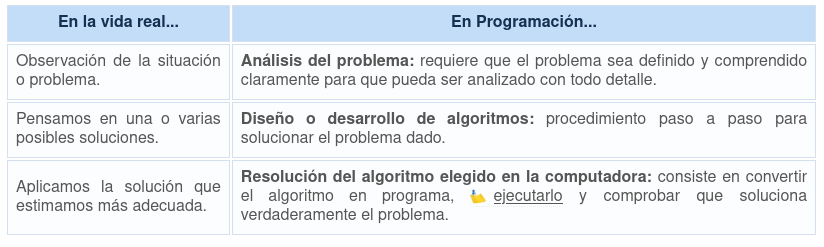
\includegraphics[scale=0.70]{pasos-problemas.png}
    \caption{Pasos para la resolución de un problema}
\end{figure}

Para que una \textbf{solución} se considere \textbf{correcta} tiene que tener principalmente dos características:

\begin{itemize}
    \item \textbf{Corrección y Eficacia}: si resuelve el problema de forma adecuada.
    \item \textbf{Eficiencia}: si lo realiza en un tiempo mínimo y con un uso óptimo de los recursos del sistema.
\end{itemize}

Para construir esta solución, hay que tener en cuenta algunos conceptos ligados a la programación, como son:

\begin{enumerate}
    \item \textbf{Abstracción}: se trata de realizar una análisis del problema para descomponerlo en problemas más pequeños y de menos complejidad de manera precisa. \textbf{Divide y Vencerás}: es una filosofía general para resolver problemas y de aquí que no solo forme parte del vocabulario informático, sino que también se utiliza en otros muchos ámbitos.

    \item \textbf{Encapsulación}: consiste en ocultar la información de un objeto o función de forma que se pueda implementar de diferentes maneras sin que esto afecte al resto de objetos.

    \item \textbf{Modularidad}: estructuraremos cada parte en módulos independientes, cada uno con su función correspondiente.
\end{enumerate}

Todo estos conceptos, deberemos tenerlos en cuenta a la hora de analizar el problema, para llegar a un solución lo más óptima posible.

\subsection{Algoritmos y Programas}
Una vez realizado el análisis del problema, tenemos que diseñar y desarrollar un \textbf{algoritmo} adecuado que pueda solucionarlo. Pero, ¿que es un algoritmo?

Un \textbf{algoritmo} es una secuencia ordenada de pasos, descrita sin ambigüedades, que conducen a la solución de un problema.

Los algoritmos deben ser \textbf{independientes} de los \textbf{lenguajes de programación} y de las \textbf{computadoras} donde se ejecutan, de forma que puedan implementarse sobre cualquier ordenador empleando cualquier lenguaje de programación. Esto facilita que una misma solución pueda emplearse para el mismo problema en diferentes dispositivos.

La \textbf{diferencia} entre un algoritmo y un \textbf{programa} es que en este último lo pasos deben escribirse en un \textbf{lenguaje de programación concreto} para que pueda ser ejecutado en el ordenador y así obtener la solución deseada.

Los \textbf{lenguajes de programación} son solo un medio para expresar el algoritmo y el ordenador un procesador para ejecutarlo. El diseño de algoritmos es una tare que requiere de la creatividad y conocimientos de las técnicas de programación del programador, así, diferentes programadores pueden desarrollar diferentes algoritmos para resolver un mismo problema.

Las principales \textbf{características} que debe cumplir un \textbf{algoritmo} son:

\begin{itemize}
    \item Debe ser \textbf{preciso} e indicar el orden en el que se realiza cada paso.
    \item Debe estar \textbf{bien definido}, si se ejecuta dos o más veces, debemos obtener el mismo resultado.
    \item Debe ser \textbf{finito}, teniendo un número de pasos bien determinado.
\end{itemize}

Cuando los problemas complejos, debemos descomponer estos en subproblemas más simples, y estos a su vez en otros más pequeños. Es lo que se conoce como \textbf{diseño descendente} o \textbf{diseño modular} y se basa en el lema \textbf{Divide y Vencerás}.

Para \textbf{representar gráficamente} los algoritmos tenemos diferentes herramientas que nos ayudarán a describir su comportamiento de una forma precisa y genérica, que nos facilitará la implementación del algoritmo en diferentes lenguajes de programación. Las principales herramientas que tenemos son:

\begin{itemize}
    \item \textbf{Diagramas de Flujo}: esta técnica utiliza símbolos gráficos para representar el flujo de ejecución del algoritmo y suelen ser empleados en la fase de análisis.
    \item \textbf{Pseudocódigo}: se basa en el uso de palabras clave en lenguaje natural, representando las constantes, variables y otras estructuras de programación de forma escrita. Es la técnica mas utilizada actualmente.
    \item \textbf{Tablas de Decisión}: es un tabla que representa las diferentes condiciones del problema con sus respectivas acciones. Suele ser una técnica de apoyo a pseudocódigo cuando existen circunstancias condicionales complejas.
\end{itemize}

\section{Fases de la Programación}
Sea cual sea el estilo que escojamos para resolver el problema, deberemos realizar el proceso aplicando un método a nuestro trabajo. Así, el \textbf{proceso de creación de software} se puede dividir en las siguientes \textbf{fases}:

\begin{itemize}
    \item \textbf{Fase de resolución del problema}
    \item \textbf{Fase de implementación}
    \item \textbf{Fase de explotación y mantenimiento}
\end{itemize}

En los siguientes puntos, analizaremos cada una de estas fases.

\subsection{Resolución del Problema}
Esta es la primera fase del desarrollo del programa, para la cuál deberá estar bien definido cual es el problema que se quiere solucionar y tener un comprensión clara de éste para poder realizar su análisis y diseño. Esta fase se puede dividir en \textbf{dos etapas}:

\begin{enumerate}
    \item \textbf{Etapa de Análisis}:

    En esta primera etapa se debe analizar el problema, lo que nos va a indicar las especificaciones y requisitos que la aplicación debe cumplir. Para llevar esto acabo, se deberán realizar diferentes entrevistas entre el programador y el cliente/usuario para precisar cuales son las características que debe tener la aplicación, especificando, entre otras cosas, los procesos y estructuras que deberá tener ésta. La creación de \textbf{prototipos} será muy útil en esta fase para saber con mayor exactitud los puntos a tratar.

    Esta etapa proporcionará una idea general de lo que se solicita, realizando sucesivos refinamientos posteriormente que servirá para determinar cual es la información que ofrecerá la resolución del problema y que datos son necesarios para resolver este.

    \item \textbf{Etapa de Diseño}:

    En esta tapa se convierte la especificación de la etapa de análisis en un diseño más detallado que define el comportamiento o la secuencia lógica de instrucciones capaz de resolver el problema planteado. Estos pasos sucesivos, constituyen lo que ya hemos definido como algoritmo.

    Antes de pasar a la implementación del algoritmo, tenemos que tener claro que la solución que se propone es la adecuada. Para ello, toda solución necesitará de la \textbf{prueba} o \textbf{traza} del programa. Este procedimiento consistirá en el seguimiento paso a paso de cada instrucción del algoritmo utilizando los datos correctos. Si la solución aportada contiene errores, deberemos volver a la etapa de análisis, si no, podremos pasar a la fase de implementación.
\end{enumerate}

\subsection{Implementación}
Esta fase consiste en plasmar en un código la solución a la que hemos llegado en la fase de resolución del problema y consta de las siguientes etapas:

\begin{enumerate}
    \item \textbf{Etapa de Codificación}:

    Esta etapa consiste en transformar o traducir la solución a la que hemos llegado en un lenguaje de programación concreto. Para comprobar la estabilidad y calidad de la solución, deberemos realizar una serie de pruebas para comprobar que los módulos funcionan correctamente (\textbf{pruebas unitarias}), que dichos módulos funcionan bien entre ellos (\textbf{pruebas de interconexión}) y todo el conjunto funciona correctamente (\textbf{pruebas de integración}).

    Cuando realizamos la traducción deberemos tener en cuenta la reglas gramaticales y sintácticas del lenguaje de programación que estemos usando, lo que generará lo que se conoce como \textbf{código fuente}, es decir, el programa en sí mismo. Pero para que nuestro programa funcione correctamente, antes deberá ser traducido a \textbf{código máquina}, el único lenguaje que entiende el ordenador. Este proceso de traducción será llevado a cabo por un \textbf{compilador} o un \textbf{interprete}, dependiendo del lenguaje de programación que estemos empleando.

    Algunos de los términos que están asociados a esta fase son los siguientes:

    \begin{itemize}
        \item \textbf{Compilación}: proceso mediante el cual el código fuente, es decir, el conjunto de instrucciones escritas en un determinado lenguaje de programación, es traducido a código máquina, un código binario que es el único lenguaje que entiende el computador.

        \item \textbf{Compilador}: es la aplicación informática que se encarga de realizar la traducción. Esta recibe el código fuente, y tras realizar una análisis lexicográfico, semántico y sintáctico, generando en primer lugar un código intermedio sin optimizar, el cual se optimiza y genera el código objeto para la plataforma especifica.

        \item \textbf{Interprete}: aplicación informática capaz de analizar y traducir programas escritos en un determinado lenguaje de programación. A diferencia de los compiladores, que realizan una traducción completa del programa a lenguaje máquina, los interpretas van realizando la traducción a medida que va siendo necesaria, típicamente, realizándola instrucción por instrucción. Además, no suelen guardar los resultados de dicha traducción.
    \end{itemize}

    \item \textbf{Prueba, Ejecución y Validación}:

    Una vez que el programa ha sido codificado, estará listo para ser ejecutado. Para ello, deberemos implantar la aplicación en el sistema donde va a ser ejecutado para comprobar su funcionamiento correcto. Utilizando diferentes datos, se comprobará si el programa cumple con los requisitos que se han especificado, si se detectan nuevos errores o si la interfaz es amigable. Se trata de poner a prueba nuestro programa para ver su respuesta en diferentes situaciones.

    Mientas que el programa tenga errores, no podremos pasar a la siguiente fase. Una vez que se corrijan, se habrán generado diferentes documentos sobre la aplicación que entrarán el alguna de las siguientes dos categorías:

    \begin{itemize}
        \item \textbf{Documentación Interna}: encabezados, descripciones, declaraciones del problema y comentarios que se incluyen dentro de código fuente.

        \item \textbf{Documentación Externa}: son los manuales que se crean para una mejor ejecución y utilización del programa, así como los diferentes diagramas generados durante el proceso de desarrollo que nos ayuden a comprender mejor su funcionamiento y arquitectura.
    \end{itemize}
\end{enumerate}

\subsection{Explotación}
En esta última fase, el software ya esta instalado en el sistema y esta siendo de utilidad para los usuarios, siendo esta la \textbf{etapa de explotación}.

Periódicamente será necesario realizar evaluaciones y, si es necesario, llevar a cabo modificaciones para que el programa se adapte o actualice a las nuevas necesidades de los usuarios, pudiendo también realizarse la corrección de errores no detectados anteriormente. Esta es la \textbf{etapa de mantenimiento}.

Así, se define el \textbf{mantenimiento de software} como el proceso de mejora y optimización del software después de su entrega al usuario final. Involucra la realización de cambios para corregir defectos y dependencias encontradas durante su uso o para la adición de funcionalidades para mejorar su usabilidad y aplicabilidad.

Sera indispensable que se haya generado la documentación adecuada para facilitar la labor del programador en la compresión, uso y modificación de la aplicación.

\section{Ciclo de Vida del Software}
Sean cuales sean las fases que las fases en las que realicemos el proceso de desarrollo de software, siempre habrá que aplicar un \textbf{modelo de ciclo vida}, siendo este una sucesión de estados o fases por las cuales pasa el software a lo largo de su vida.

Este proceso debe tener siempre la siguientes etapas mínimas:

\begin{itemize}
    \item \textbf{Especificación} y \textbf{Análisis de Requisitos}
    \item \textbf{Diseño}
    \item \textbf{Codificación}
    \item \textbf{Pruebas}
    \item \textbf{Instalación} y \textbf{Producción}
    \item \textbf{Mantenimiento}
\end{itemize}

Existen diferentes modelos de desarrollo como el modelo en cascada, en espiral, incremental, evolutivo, etc.. En la siguiente \href{https://es.wikipedia.org/wiki/Proceso_del_desarrollo_del_software}{entrada de Wikipedia} podemos ver más información sobre el proceso de desarrollo de software y las diferentes metodologías.

\section{Lenguajes de Programación}
Como hemos visto en los puntos anteriores, una de las etapas del desarrollo es la codificación del programa. Para ello, emplearemos un lenguaje que exprese cada uno de los pasos que se deben ejecutar. Este lenguaje recibe el nombre de \textbf{lenguaje de programación}.

Se entiende por \textbf{lenguaje de programación} el conjunto de reglas sintácticas y semánticas, símbolos y palabras especiales establecidos para la construcción del programa. Todo lenguaje se compone de:

\begin{itemize}
    \item \textbf{Gramática}: reglas aplicables al conjunto de símbolos y palabras empleados en el lenguaje de programación para la construcción de sentencias correctas.
    \item \textbf{Léxico}: es el conjunto de símbolos y palabras especiales, es decir, el vocabulario del lenguaje.
    \item \textbf{Sintaxis}: son las posibles combinaciones de símbolos y palabras especiales.
    \item \textbf{Semántica}: es el significado de cada construcción del lenguaje, es decir, la acción que se llevará a cabo.
\end{itemize}

Los lenguajes permiten que los programadores pueden expresar el código de forma que sea legible para ellos y otros programadores. Estos se clasifican según lo cercanos que estén al lenguaje máquina o al lenguaje natural, así como si son lenguajes interpretados o compilados, lo que vamos a ver en los siguientes puntos.

\subsection{Lenguaje Máquina}
Este lenguajes es él único que entiende el ordenador y se compone de un conjunto de instrucciones codificadas en binario que se encarga de ejecutar el procesador. Este lenguaje es directamente interpretable por un circuito microprogramable.

Se trata del primer lenguaje utilizado para la programación de computadoras. De hecho, cada máquina tenía su propio conjunto de instrucciones codificadas en ceros y uno. Esto, evidentemente, genera un conjunto de \textbf{inconvenientes}:

\begin{itemize}
    \item Cada programa era válido \textbf{solo para un tipo de procesador} u ordenador.
    \item La \textbf{lectura} e \textbf{interpretación} de este tipo de programas es \textbf{extremadamente difícil}, por lo que realizar modificaciones resultaba extremadamente costoso.
    \item Los programadores de la época debían \textbf{memorizar largas cadenas de unos y ceros}, que equivalían a las instrucciones disponibles en los diferentes tipos de procesadores.
    \item Además, la introducción de estas cadenas suponía \textbf{largos tiempos de espera y posibles errores}.
\end{itemize}

En la siguiente tabla muestran algunos ejemplos de operaciones codificadas en binario.

\begin{figure}[H]
    \centering
    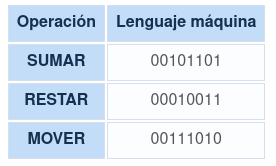
\includegraphics[scale=1]{ejemplo-binario.png}
    \caption{Operaciones en binario}
\end{figure}

Dada la dificultad de este lenguaje, con el tiempo fue sustituido por otros de más fácil compresión, aunque hay que tener en cuenta que en última instancia todos los lenguajes deben ser traducido a éste para que puedan ser interpretados y ejecutados por el ordenador.

\subsection{Lenguaje Ensamblador}
La evolución del lenguaje máquina fue el \textbf{lenguaje ensamblador}. En éste, las instrucciones ya no son secuencias binarias sino que son códigos de operación que describen operaciones básicas del procesador.

Estos códigos, conocidos como \textbf{mnemotécnicos}, son palabras especiales que sustituyen largas secuencias de unos y ceros, utilizadas para referirse a diferentes operaciones disponibles en el juego de instrucciones que soporta un procesador concreto.

En la siguiente tabla, podemos ver alguno ejemplos de estos mnemotécnicos con diferentes operaciones.

\begin{figure}[H]
    \centering
    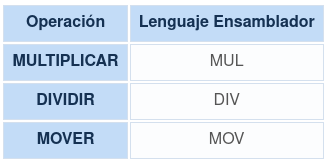
\includegraphics[scale=1]{ejemplo-asm.png}
    \caption{Operaciones en ensamblador}
\end{figure}

Aunque el ensamblador fue un intento de acercar el lenguaje máquina al lenguaje humano, aún presentaba diferentes \textbf{dificultades}:
\begin{itemize}
    \item Los programas seguían \textbf{dependiendo} directamente del \textbf{hardware} que los soportaba.
    \item Los programadores debían \textbf{conocer} detalladamente \textbf{la máquina} sobre la que programaban, ya que debían hacer un uso adecuado de los recursos del sistema.
    \item La \textbf{lectura}, \textbf{interpretación} o \textbf{modificación} de los programas seguía presentando dificultades.
\end{itemize}

Todo programa escrito en ensamblador necesita ser traducido al lenguaje máquina para poder ser ejecutad. Esta función la lleva a cabo el \textbf{programa ensamblador}, el cual convierte el programa original escrito en lenguaje ensamblador (código fuente) en el programa traducido a lenguaje máquina (código objeto).

\subsection{Lenguajes Compilados}
% Bibliography

\newpage
\addcontentsline{toc}{chapter}{Bibliografía}
\bibliography{citas}
\bibliographystyle{unsrt}

\end{document}